% !TEX root = PREN2_Dokumentation.tex
\section{System-Spezifikation}\label{SystemSpezifikation}
\subsection{Systemübersicht}
\subsubsection{Systemarchitektur}
\begin{figure}[H]
    \centering
    \includegraphics[width=1\textwidth]{images/systemoverview.png}
    \caption[Systemarchitektur]{Systemarchitektur,\\ Quelle: Autoren}
    \label{img: Systemarchitektur des Projektes}
\end{figure}
\newpage
\subsubsection{Kontextdiagram}\label{Kontextdiagram}
\begin{figure}[H]
    \centering
   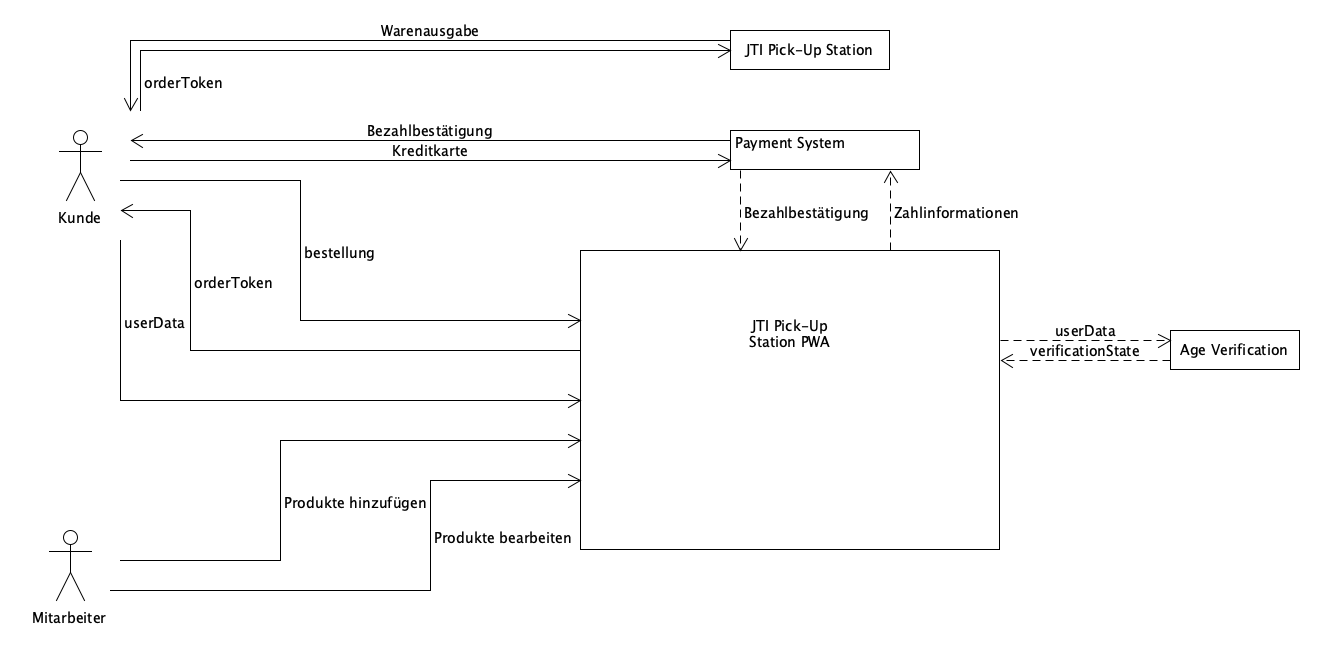
\includegraphics[width=1\textwidth]{images/kontextdiagramm.png}
    \caption[Kontextdiagramm]{Kontextdiagramm,\\ Quelle: Autoren}
    \label{img: Kontextdiagramm des Projektes}
\end{figure}
\newpage


\newpage
\subsection{Architektur und Designentscheide}
Es wurde bei diesem Projekt auf eine REST-Architektur gesetzt. Die Web-Applikation wird als \ac{PWA} umgesetzt. 
\subsubsection{Modelle und Sichten}
In diesem Projekt wird zwischen zwei verschiedenen Sichten unterschieden:
\begin{itemize}
    \item \textbf{Kunde} Es handelt sich dabei um die Person, welche in der \ac{PWA} Produkte bestellt und diese anschliessend abholt. 
    \item \textbf{Administrator} Dem Administrator ist es möglich, Produkt hinzuzufügen, zu verändern oder auch zu löschen. 
    \item \textbf{Programmierer: } Dieser konzipiert und realisiert die Applikation gemäss den Anforderungen des Auftraggebers.
\end{itemize}
\subsubsection{Daten (Mengengerüst und Strukturen)}
\paragraph{Datenbankschema}
Das Datenbankschema wurde mittels Reverse Engineering erstellt und ist in der Abbildung \ref{img: datebankschema} ersichtlich.
\begin{figure}[H]
    \centering
    %\includegraphics[width=1\textwidth]{bilder/datenbankschema.png}
    \caption[Datenbankschema]{Datenbankschema, Quelle: Autoren}
    \label{img: datebankschema}
\end{figure}
\subsubsection{Entwurfsentscheide}
\paragraph{Frontend}
\subparagraph{Technologien}
Das Frontend wurde mit React aufgebaut, wobei als Hilfsmittel \cite{create-react-app} für die Entwicklung verwendet wurde.
Betrieben wird die Applikation auf einem NGINX-Webserver mit der Version 1.16.0, welcher durch die \cite{create-react-app} mitgeliefert wird.
\subparagraph{Projektstruktur}
\begin{wrapfigure}{r}{5.5cm}
    %\includegraphics[width=5.5cm]{bilder/strukturreactfrontend.png}
    \caption{Projektstruktur vom Frontend}\label{img: reactprojectstructure}
\end{wrapfigure}
Die Projektstruktur ist wie folgt gegliedert:
\begin{itemize}
    \item Components: Darin befinden sich alle Komponenten welche für die Applikation aufgebaut wurden.
    \begin{itemize}
        \item Frontpage: Komponenten welche ohne Authentifizierung zugänglich sind.
        \item MainContent: Komponenten die nur durch eine erfolgreiche Authentifizierung zugänglich sind.
        \begin{itemize}
            \item Admin: Komponenten für die Lehrer als auch Administratoren (bspw. Formulare, Im- und Exports etc.)
            \item Exam: Komponenten welche für die Prüfungen zuständig sind.
            \item MainComponents: Komponenten welche alle durch den Schüler zugänglich und die Mainfeatures ausmachen wie bspw. das Quiz, die Statistiken etc.
            \item Navigation: Der Inhalt der Sidebar als auch diverse Navigationshilfsmittel.
            \item Utils: Diverse Hilfsmittel
            \item MainContent: Dabei handelt es sich um die Hauptkomponente bei der bspw. der Router eingebaut ist und somit anhand der URL die entsprechende Komponenten rendert.
        \end{itemize}
        \item Quiz: Hierbei handelt es sich um die Quiz-Komponente, welche für die Übungen verwendet wird.
    \end{itemize}
    \item CSS: Darin sind alle Stylesheets welche nicht in den Komponenten direkt eingebaut wurden.
    \item images: Hier befinden sich alle Bilder welche für das Frontend verwendet wurden.
    \item Redux: Hier befinden sich alle Redux-Komponenten, welche alle Reducers, Actions und den Store beinhalten.
    \item AuthService. Hier wurden alle Services zusammengefasst, welche einerseits mit der Authentifizierung als auch mit der API vom Backend etwas zu tun haben.
\end{itemize}
In der Abbildung \ref{img: componentdiagram} ist ein vereinfachtes Komponentendiagramm ersichtlich, welches die selbst entwickelten Komponenten aufweist.
\begin{figure}[H]
    \centering
   % \includegraphics[width=1\textwidth]{bilder/componentdiagram.png}
    \caption[Komponentendiagramm des Frontends]{Komponentendiagramm des Frontends, Quelle: Autoren}
    \label{img: reactcomponents}
\end{figure}

\subparagraph{Externe Packages}
In der Abbildung \ref{img: reactdependencies} sind alle externen Packages aufgelistet, welche für dieses Projekt verwendet wurden.
\begin{figure}[H]
    \centering
   % \includegraphics[width=1\textwidth]{bilder/reactdependencies.png}
    \caption[Externe Packages für das Frontend]{Externe Packages für das Frontend, Quelle: Autoren}
    \label{img: reactdependencies}
\end{figure}

\paragraph{Backend}
\subparagraph{Spring Boot}
Für die Backendentwicklung wurde Spring Boot in der Version 2.3.4 genutzt.
\paragraph{Datenbank}
Als Datenbank wurde während der Entwicklung MariaDB in der Version 10.5 genutzt.
Für die Auslieferung der Applikation wurde auf Postgre SQL gewechselt.
\paragraph{Konfigurationen}
\subparagraph{Frontend}
An folgenden Dateien können Konfigurationen am Frontend vorgenommen werden:
\begin{itemize}
    \item nginx.config: Dort kann Webserver-Konfigurationen für den nginx vorgenommen werden. Falls ein anderer Webserver verwendet wird, ist diese Konfiguration überflüssig.
    \item package.json: Darin werden alle Abhängigkeiten und externen Packages verwaltet inklusive deren Versionierung.
    \item Dockerfile: Hier wird der Container-Build deklariert wobei hier auch diverse Einstellungen wie bspw. das Einbinden eines Zertifikats oder weitere Konfigurationen am Nginx vorgenommen werden können.
\end{itemize}
\newpage
\subparagraph{Backend}
Die Konfigurationen im Backend wurden mittels des application.propertie-File gemacht.
\begin{verbatim}
spring.jpa.hibernate.ddl-auto=update

#for development with mariadb
#spring.datasource.url=jdbc:mariadb://mariadb:3306/db_electrolernapp?
createDatabaseIfNotExist=true
#spring.datasource.url=jdbc:mariadb://localhost:3306/db_electrolernapp?
#spring.datasource.username=root
#spring.datasource.password=electrolernapp2020

#for development with postgresql
spring.datasource.url=jdbc:postgresql://localhost:5432/db_electrolernapp?
createDatabaseIfNotExist=true
spring.datasource.username=elektro_app_user
spring.datasource.password=j^\k&hKbm8A!n2"]
spring.datasource.driver-class-name=org.mariadb.jdbc.Driver
spring.hateoas.use-hal-as-default-json-media-type=true
spring.jackson.time-zone: Europe/Paris
spring.http.multipart.max-request-size=50Mb

# CSV Configurations
spring.servlet.multipart.max-file-size=10MB
spring.servlet.multipart.max-request-size=10MB


# App Properties
bezkoder.app.jwtSecret= bezKoderSecretKey
bezkoder.app.jwtExpirationMs= 86400000

server.contextPath=/api/v1
springfox.documentation.swagger.v2.path=/api-docs

#Mail properties
spring.mail.host=smtp.gmail.com
spring.mail.port=587
spring.mail.username=electrolernapp@gmail.com
spring.mail.password=electrolernapp2020
spring.mail.smtp.auth=true
spring.mail.properties.mail.smtp.auth=true
spring.mail.properties.mail.smtp.starttls.enable=true

\end{verbatim}
\newpage
\subsection{Schnittstellen}

\subsubsection{Externe Schnittstellen}
\paragraph{REST API}
Die REST-Schnittstelle wurde mit dem Tool \glqq Swagger\grqq{} erstellt.
Die Dokumentation ist im Anhang im Kapitel \ref{SwaggerDokumentation} aufzufinden.
\subsubsection{Wichtige interne Schnittstellen}


\paragraph{CsvService}
\subparagraph{Steckbrief}
Die Schnittstelle \glqq CsvService\grqq{} dient dazu, Entities über eine CSV-Datei in die Datenbank zu migrieren.
\subparagraph{Interaktionen}
\paragraph{Operationen und Datenstrukturen}
\begin{figure}[H]
    \centering
    %\includegraphics[width=7cm]{bilder/csvservice.png}
    \caption[Klassendiagramm des CsvParsers]{Klassendiagramm des CsvParsers, Quelle: Autoren}
    \label{img: csvservice}
\end{figure}

\subparagraph{Einsatz, Abläufe, Voraussetzungen und Zusicherung}
\begin{itemize}
    \item Bei der Implementation einer Klasse mit der Verwendung dieser Schnittstelle ist es jeweils notwendig, die Repsitory-Klasse der betroffenen Entities, welche vom JpaRepository erben, zu injecten.
    \item Der Header der CSV-Datei muss von vornherein klar definiert werden und ist nicht dynamisch anpassbar.
\end{itemize}

\subparagraph{Aufbau und Konfiguration}
Keine zusätzlichen Informationen.
\subparagraph{Fehlerbehandlung}
Zur Fehlerbehandlung werden Runtime Exceptions geworfen, wenn eine CSV-Datei nicht eingelesen werden kann.
Es können aber auch ResourceNotFoundExceptions auftreten, wenn Entities Abhängigkeiten zu anderen Entities haben, die jedoch nicht gefunden werden.
Wichtig ist, dass die Exceptions auf jeden Fall geworfen werden, damit der CsvController den Clients eine entsprechende Rückmeldung geben kann und den Prozess beendet.

\subparagraph{Qualitätsmerkmale}
Keine zusätzlichen Informationen.
\subparagraph{Entwurfsentscheidungen}
\begin{itemize}
    \item Die Schnittstelle besitzt eine default-Methode, um den Typ der Datei zu überprüfen.
    \item Diese Schnittstelle wurde darauf ausgelegt, lediglich mit CSV-Dateien zu arbeiten. Für andere Dateitypen sollte eine neue Schnittstelle definiert werden.
\end{itemize}

\subparagraph{Beispielverwendung}
\begin{verbatim}
//Injection im CsvController
@Autowired
private CsvCategoryService csvCategoryService;

//Einsatz des CsvControllers
if (csvCategoryService.hasCSVFormat(categoryFile)) {
            try {
                csvCategoryService.saveNewEntities(categoryFile);

                categoryMessage = "Uploaded the file successfully: " +
                categoryFile.getOriginalFilename();
                messageList.add(new MessageResponse(categoryMessage));
            } catch (Exception e) {
                categoryMessage = "Could not upload the file: " + 
                categoryFile.getOriginalFilename() +
                 "! " + e.getMessage();
                LOG.error(categoryMessage);
                e.printStackTrace();
                messageList.add(new MessageResponse(categoryMessage));
                return ResponseEntity.status(HttpStatus.EXPECTATION_FAILED)
                .body(messageList);
            }
}
\end{verbatim}
\newpage
\paragraph{DTOParser}
\subparagraph{Steckbrief}
Als interne Schnittstelle kommt die DTOParserStrategy bei der Übersetzung von Data Transfer Objects zu Entities zum Einsatz.
Diese befindet sich in der Version 1.0.0.
\subparagraph{Interaktionen}
\paragraph{Operationen und Datenstrukturen}
\begin{figure}[H]
    \centering
   % \includegraphics[width=11cm]{bilder/dtoStrategy.png}
    \caption[Klassendiagram DTOStrategy Question]{Klassendiagram DTOStrategy Question, Quelle: Autoren}
    \label{img: dtoStrategy}
\end{figure}
\subparagraph{Einsatz, Abläufe, Voraussetzungen und Zusicherung}
\begin{itemize}
	\item Bevor die Schnittstelle verwendet werden kann, muss der dazugehörige Service mittels Autowired in die betreffende Klassen injected werden.
	\item Die eingegebene Id muss mit einem der Datenbankobjekte übereinstimmen.
\end{itemize}
\subparagraph{Aufbau und Konfiguration}
Keine zusätzlichen Informationen.
\subparagraph{Fehlerbehandlung}
Zur Fehlerbehandlung werden Runtime Exceptions geworfen, wenn ein Element beim Parsen nicht verfügbar ist.

\subparagraph{Qualitätsmerkmale}
Keine zusätzlichen Informationen.
\subparagraph{Entwurfsentscheidungen}
\begin{itemize}
\item Die Schnittstelle wurde mit Generics umgesetzt, um sie für alle Parser verwenden zu können.
\item Mit den hier vorgegebenen Interfaces können beliebige Typen mitgegeben und auch zurückgeben werden.
\end{itemize}

\begin{figure}[H]
	\centering
	%\includegraphics[width=10cm]{bilder/package.png}
	\caption[Packagediagram Backend]{Packagediagram Backend, Quelle: Autoren}
	\label{img: package}
\end{figure}

\subparagraph{Beispielverwendung}
\begin{verbatim}
//Parsen von Listen
dtoParserQuestion.generateDTOsFromObjects(questions);

//Parsen von einzelnem Element
dtoParserQuestion.generateDTOFromObject(question.getId());

//Parsen von Objekt zu DTO
Question question = dtoParserQuestion.generateObjectFromDTO(questionDTO);
\end{verbatim}

\subsubsection{Benutzerschnittstellen}
Als Benutzerschnittstelle fungiert hierbei lediglich das Frontend.
Hierfür werden zwei Bereiche unterschieden:
\begin{itemize}
    \item Öffentlicher Bereich: In diesem Bereich erscheint der Benutzer beim Aufruf der Website und ist für jedermann zugänglich.
    \item Privater Bereich: In diesem Bereich kann sich ein Benutzer lediglich befinden, wenn dieser sich erfolgreich authentifiziert hat.
\end{itemize}

\paragraph{Öffentlicher Bereich}
In diesem Bereich steht den Benutzern folgende drei Formulare zur Verfügung:
\begin{itemize}
    \item Login: Hier kann sich ein Benutzer mit seinem Benutzernamen sowie seinem Passwort einloggen. Von hier aus kann dieser auf den Reiter \glqq Passwort zurücksetzen\grqq wechseln.
    \item Passwort zurücksetzen: Hier kann der Benutzer seine E-Mail-Adresse eingeben um sein Passwort zurücksetzen zu lassen.
    \item Passwort neu setzen: Hier muss der Benutzer das neue Passwort zwei Mal eingeben. Dieses Formular kann lediglich mit einem gültigen Token im Backend abgearbeitet werden.
\end{itemize}
\newpage
\paragraph{Privater Bereich}
In diesem Bereich wird zwischen der Schülersicht sowie der Lehrersicht unterschieden.
Der Lehrer besitzt dieselbe Sicht wie der Schüler.
Es stehen ihm aber auch noch zusätzliche Features zur Verfügung.
Die Sichten beziehen sich dabei auf die Abbildung \ref{img: lehrersicht}.


\subparagraph{Schülersicht}
Dem Schüler stehende folgende Sichten zur Verfügung:
\begin{enumerate}
    \item Home: Hier kann der Benutzer jederzeit auf die Startseite der Applikation navigieren.
    \item Übungen: Darin kann sich der Benutzer durch die Kategorien sowie Übungssets navigieren und ein solches starten.
    \item Prüfungen: In der Prüfungsübersicht kann der Benutzer seine anstehenden als auch absolvierten Prüfungen betrachten.
    \item Statistiken: Hier kann der Benutzer seine eigenen Statistiken in Bezug auf alle Kategorien als auch auf die einzelnen Übungssets betrachten.
    \setcounter{enumi}{11}
    \item Profil: Hier kann man das eigene Profil betrachten, welces aus dem Benutzernamen und der E-Mail-Adresse besteht.
\end{enumerate}

\begin{figure}[H]
    \centering
   % \includegraphics[width=1\textwidth]{bilder/lehrersicht.png}
    \caption[Lehrersicht der Applikation]{Lehrersicht der Applikation, Quelle: Autoren}
    \label{img: lehrersicht}
\end{figure}
\newpage
\subparagraph{Lehrersicht}
Während dem Lehrer dieselben Sichten wie des Schülers zur Verfügung stehen, besitzt dieser weitere welche zur Administration dienen.
\begin{enumerate}
    \setcounter{enumi}{4}
    \item Benutzerverwaltung: Bei der Benutzerverwaltung besteht die Möglichkeit entweder einen einzelnen Benutzer über ein Registrierungsformular zu erstellen oder anhand einer CSV-Datei mehrere Benutzer zu importieren.
    \item Prüfung erstellen: Hier kann anhand eines Formulars eine Prüfung erstellt werden, in dem man mehrere Fragen in eine Liste zusammenfügt.
    \item Fragen erstellen: In diesem Formular lassen sich neue Fragen erstellen und einem Übungsset zuweisen.
    \item Klasse erstellen: Hier kann man eine Klasse erstellen, indem man diese einer Bildungsinstitution zuweist und entsprechende Schüler hinzufügt.
    \item Klasse bearbeiten: Dieses Formular sieht genau gleich aus wie das bei der Erstellung der Klasse, wohingegen hier über die Wahl der Bildungsinstitution und der entsprechenden Klasse diese danach bearbeitet werden kann.
    \item Bildungsinstitution erstellen: Hiermit wird eine neue Bildungsinstitution erstellt.
    \item Daten exportieren: Hier lassen sich entsprechende Daten exportieren. Aktuell stehen Frage,, Benutzer, Prüfungen und Prüfungsergebnisse als Export zur Verfügung.
\end{enumerate}
\newpage
\subsection{Environment-Anforderungen}\label{environmentanforderungen}
Da keine ausgiebige Evaluation der Hardware- als auch Softwareplattform vorgenommen wurde, wird hier auf die Umgebung eingegangen, auf der die Applikation aufgebaut wurde und somit bestätigt werden kann, dass anhand dieser Anforderungen ein Betrieb der Applikation möglich ist.
\subsubsection{Hardware}
Folgende Hardware wurde für diese Applikation verwendet und kann als ausreichend betrachtet werden:
\begin{itemize}
    \item CPU: Intel(R) Xeon(R) CPU E5-2630 v4 @ 2.20GHz
    \item RAM: 4GB
\end{itemize}
\subsubsection{Software}
Die ganze Applikation läuft auf einer virtuellen Maschine, auf der folgendes Betriebssystem inklusive Packages installiert sind:
\begin{itemize}
    \item Ubuntu v. 20.04.01
    \item Docker v. 19.03.8
\end{itemize}
Des Weiteren musste ein SSH-Key mittels dem \glqq ssh-keygen\grqq{} generiert werden, damit das Deployment sichergestellt werden konnte.
Die SSH-Packages sind jedoch im Ubuntu bereits integriert.
\newpage